% !TeX spellcheck = fr_FR
\chapter{Chapitre 6 : Expérimentation}
\label{chap:6}

\section{PMC}
\label{sec:6.1}

\subsection{Architecture avec TFR}

\begin{figure}[H]
	\centering
	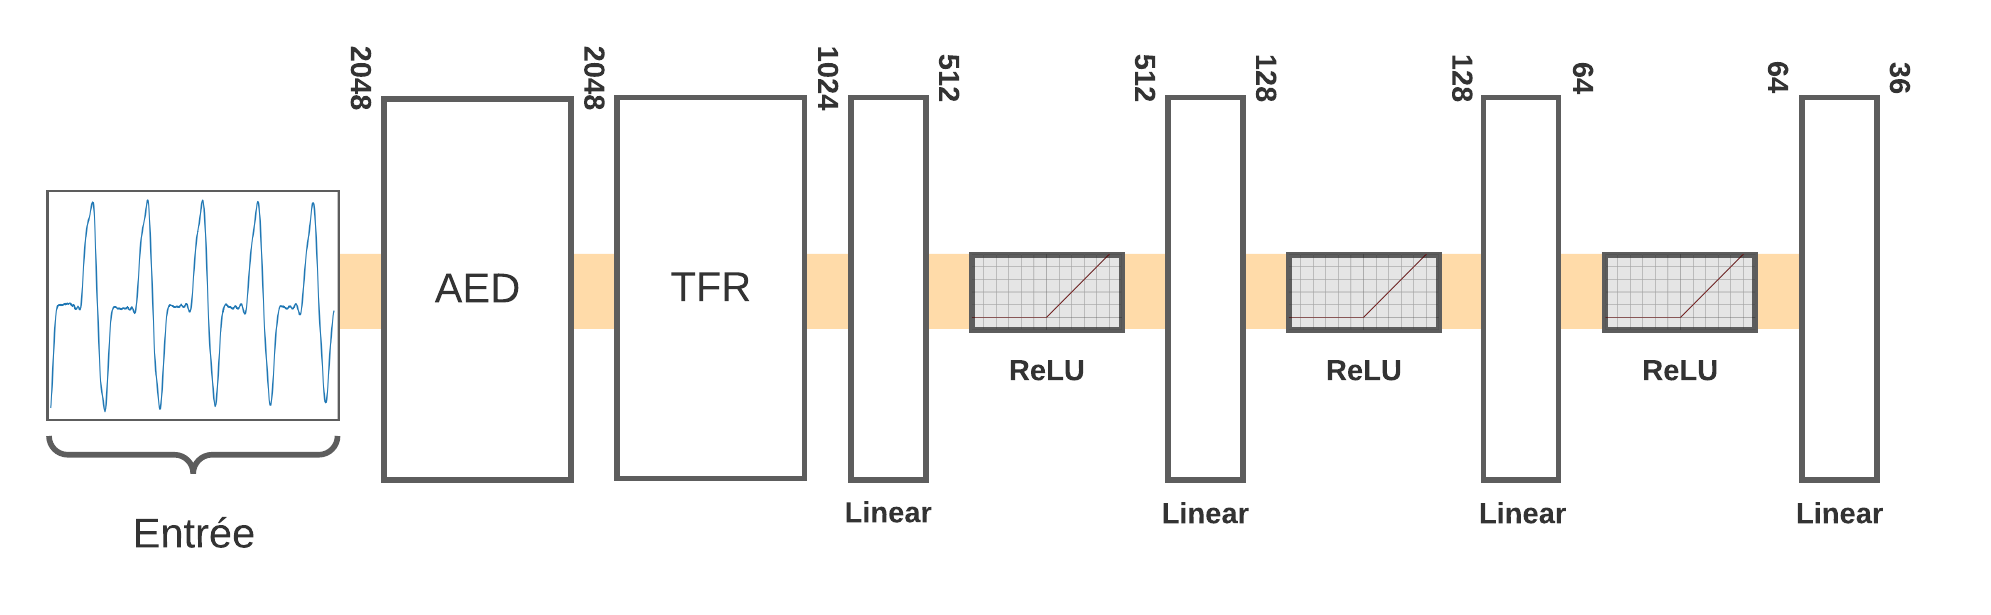
\includegraphics[width=1\linewidth]{mlp_fft}
	\caption[Architecture PMC avec TFR]{Architecture PMC avec TFR. Source : Réalisé par \textsc{Küenzi} Jean-Daniel}
	\label{fig:mlp_fft}
\end{figure}

\subsection{Matrice de confusion sur l'ensemble de validation}
\label{subsec:6.1.2}

La matrice de confusion suivante a été réalisée avec le modèle utilisant une fenêtre de 2048 échantillons.

\begin{figure}[H]
	\centering
	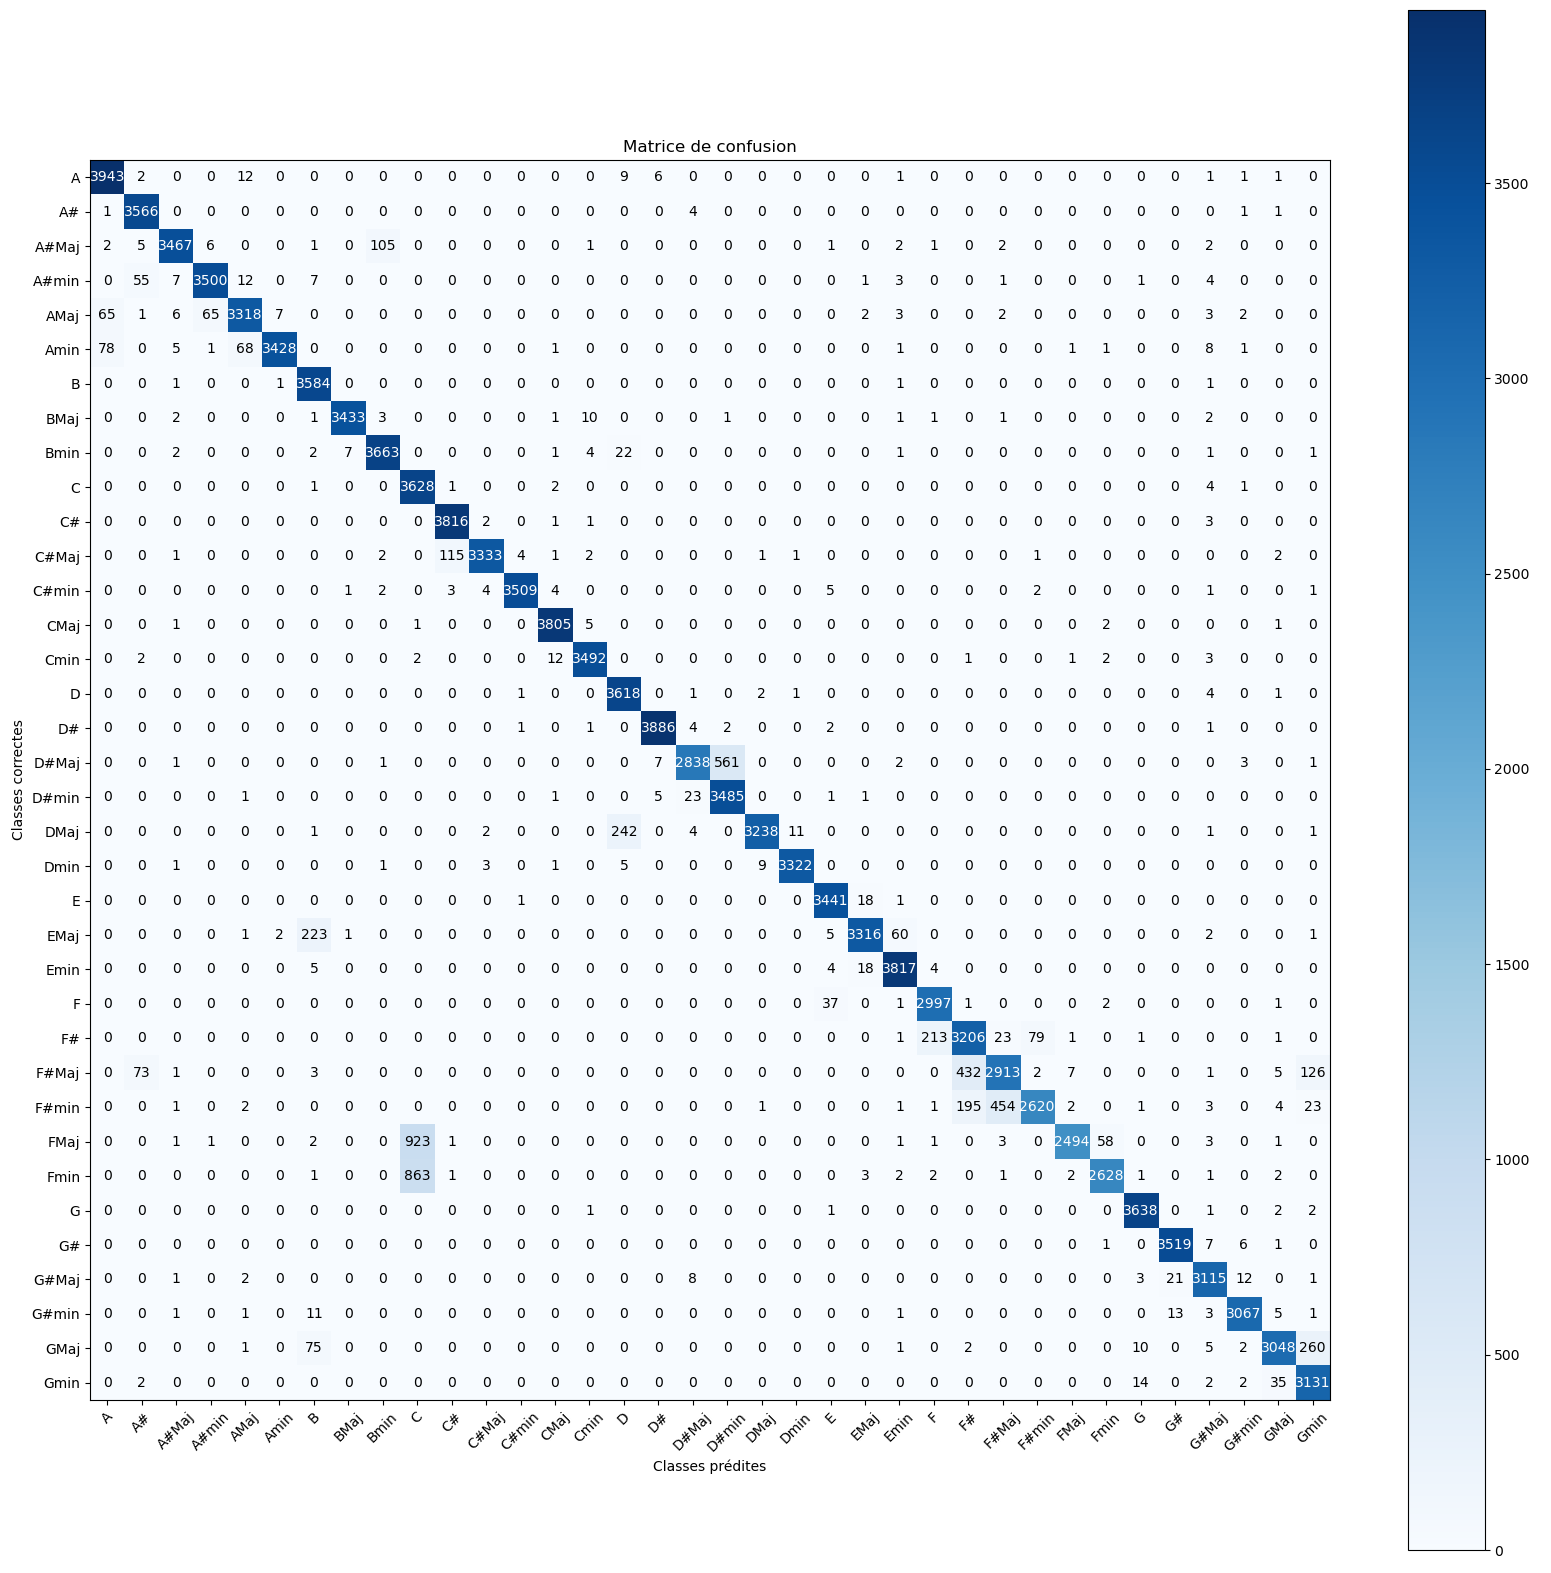
\includegraphics[width=1\linewidth]{cm_mlp_fft}
	\caption[Matrice de confusion pour l'architecture PMC avec TFR]{Matrice de confusion pour l'architecture PMC avec TFR. Source : Réalisé par \textsc{Küenzi} Jean-Daniel}
	\label{fig:cm_mlp_fft}
\end{figure}

Lorsque l'on observe cette matrice de confusion, on remarque que le modèle a l'air de s'être fortement trompé sur FMaj, Fmin, EMaj et Dmaj. En fait finalement si l'on observe bien, par exemple pour le cas de FMaj, le modèle a prédit certains exemples comme étant la note C. Ce résultat n'est pas si faux étant donné que la note C est la quinte du FMaj et Fmin (voir \autoref{sec:2.3}). Mais surtout lorsque l'on écoute le fichier FMaj2.wav de l'ensemble de validation, il s'avère qu'effectivement vers la fin de l'accord, il ne reste plus que la note C que l'on entend. Et donc ce résultat est juste. Finalement cette erreur relève d'une imperfection dans l'ensemble de validation. Fmin, EMaj et Dmaj sont dans le même cas. Vous pouvez retrouver en annexe (voir \autoref{app:4}) la prédiction du modèle sur le fichier FMaj2.wav de l'ensemble de validation.

Finalement les erreurs où, à la place d'un accord, le modèle trouve une note, à savoir soit la fondamentale, soit la tierce, soit la quinte, ne sont pas trop graves et généralement cela n'est pas réellement une erreur, mais relève d'une imperfection dans les enregistrements de l'ensemble de validation. Les erreurs les plus graves surviennent lorsque le modèle prédit une note comme étant un accord ou se trompe dans une note ou un accord de manière très éloignée de la classe correcte, par exemple F\sh\,prédit comme un F\sh min.

\subsection{Entrainements pour différentes tailles de fenêtres}

\begin{table}[H]
	\centering{
		\begin{tabular}{c l c c}
			\hline
			\multicolumn{4}{c}{\textbf{PMC avec TFR}} \\
			\multicolumn{4}{c}{epochs = 50, $\eta$ = 0.005, nombre d'entrainements = 10} \\
			\hline
			\textbf{Nombre d'échantillons} & \textbf{Données} & \textbf{Précision moyenne \%} & \textbf{Ecart type \%} \\
			\hline
			\multirow{2}{*}{1024} & Entrainement & 99.44 & 0.07 \\
			& Validation & 85.60 & 0.63 \\
			\hline
			\multirow{2}{*}{2048} & Entrainement & 99.86 & 0.03 \\
			& Validation & 95.23 & 0.80 \\
			\hline
			\multirow{2}{*}{3072} & Entrainement & 99.89 & 0.02 \\
			& Validation & 94.56 & 0.34 \\
			\hline
			\multirow{2}{*}{4096} & Entrainement & 99.90 & 0.01 \\
			& Validation & 94.65 & 0.24 \\
			\hline
		\end{tabular}
		\caption[Entrainement de l'architecture PMC avec TFR]{Entrainement de l'architecture PMC avec TFR. Source : Réalisé par \textsc{Küenzi} Jean-Daniel}
		\label{tab:pmc_with_tfr}
	}
\end{table}

Lorsque l'on observe les résultats de l'architecture \gls{pmc} avec \gls{tfr}, le premier constat est qu'une fenêtre de 1024 échantillons, soit une résolution temporelle de \textasciitilde$0.023$[s], donne de mauvais résultats avec la \gls{tfr}. Cela peut s'expliquer par la résolution fréquentielle. Avec 1024 échantillons nous avons une résolution fréquentielle de \textasciitilde$43.06$[Hz]. On peut donc facilement confondre des notes et des accords. Ensuite, le deuxième constat est qu'à partir d'une fenêtre de 2048 échantillons, augmenter le nombre d'échantillons (donc la taille de la fenêtre) n'améliore pas la précision du modèle. Elle la fait même légèrement chuté, mais cela peut être en partie dû à la réduction de la taille de l'ensemble de données ainsi que du problème évoqué dans la \autoref{subsec:6.1.2}. Donc 2048 échantillons semblent une bonne de taille fenêtre, nous avons une résolution fréquentielle de \textasciitilde$21.53$[Hz] et une résolution temporelle de \textasciitilde$0.046$[s]. Comme sa résolution temporelle est faible, cette fenêtre semble être un bon choix pour le temps réel.

De plus, les résultats sont extrêmement bons, on voit bien que le modèle arrive correctement à différencier les différents accords et notes. Même s'ils sont légèrement faussés à cause du problème évoqué dans la \autoref{subsec:6.1.2}, ses résultats restent très prometteurs et encourageants.

\begin{table}[H]
	\centering{
		\begin{tabular}{c l c c}
			\hline
			\multicolumn{4}{c}{\textbf{PMC sans TFR}} \\
			\multicolumn{4}{c}{epochs = 50, $\eta$ = 0.005, nombre d'entrainements = 10} \\
			\hline
			\textbf{Nombre d'échantillons} & \textbf{Données} & \textbf{Précision moyenne \%} & \textbf{Ecart type \%} \\
			\hline
			\multirow{2}{*}{1024} & Entrainement & 99.56 & 0.21  \\
			& Validation & 91.21 & 0.27 \\
			\hline
			\multirow{2}{*}{2048} & Entrainement & 99.88 & 0.07 \\
			& Validation & 92.34 & 0.37 \\
			\hline
			\multirow{2}{*}{3072} & Entrainement & 99.82 & 0.08 \\
			& Validation & 92.22 & 0.41 \\
			\hline
			\multirow{2}{*}{4096} & Entrainement & 99.98 & 0.03 \\
			& Validation & 91.29 & 0.11 \\
			\hline
		\end{tabular}
		\caption[Entrainement de l'architecture PMC sans TFR]{Entrainement de l'architecture PMC sans TFR. Source : Réalisé par \textsc{Küenzi} Jean-Daniel}
		\label{tab:pmc_without_tfr}
	}
\end{table}

Lorsque l'on observe les résultats de l'architecture \gls{pmc} sans \gls{tfr}, on constate tout d'abord que les résultats sont globalement plutôt bons, même s'ils sont moins bons que pour l'architecture avec \gls{tfr}. Ensuite on constate qu'à partir de la fenêtre de 2048 échantillons, la précision du modèle chute légèrement. Cela peut être expliqué par le nombre d'epochs qui n'est peut-être plus assez suffisant pour laisser au modèle le temps de converger correctement. Les résultats sans \gls{tfr} (avec les données discrètes) sont plutôt encourageants eux aussi. Bien qu'ils soient légèrement moins bons que les résultats avec \gls{tfr}, cela reste une piste à ne pas écarter et à continuer de chercher de ce côté là. Il serait en effet intéressant pour le temps réel de ne pas avoir à passer par une \gls{tfr}.

Les résultats du \gls{pmc} m'ont assez surpris, je ne m'attendais pas à autant de performance de la part de cette architecture. Mais finalement cela peut s'expliquer par le fait que le \gls{pmc} prend en entrée la composante du spectre continu, donc les différentes raies de la \gls{tfr}, et ses raies se trouveront toujours autour des mêmes neurones. De plus comme l'ensemble de données est relativement petit, le \gls{pmc} arrive finalement à apprendre la classification de chaque note et accord.

\section{RNC}
\label{sec:6.2}

\subsection{Architecture avec TFR}

\begin{figure}[H]
	\centering
	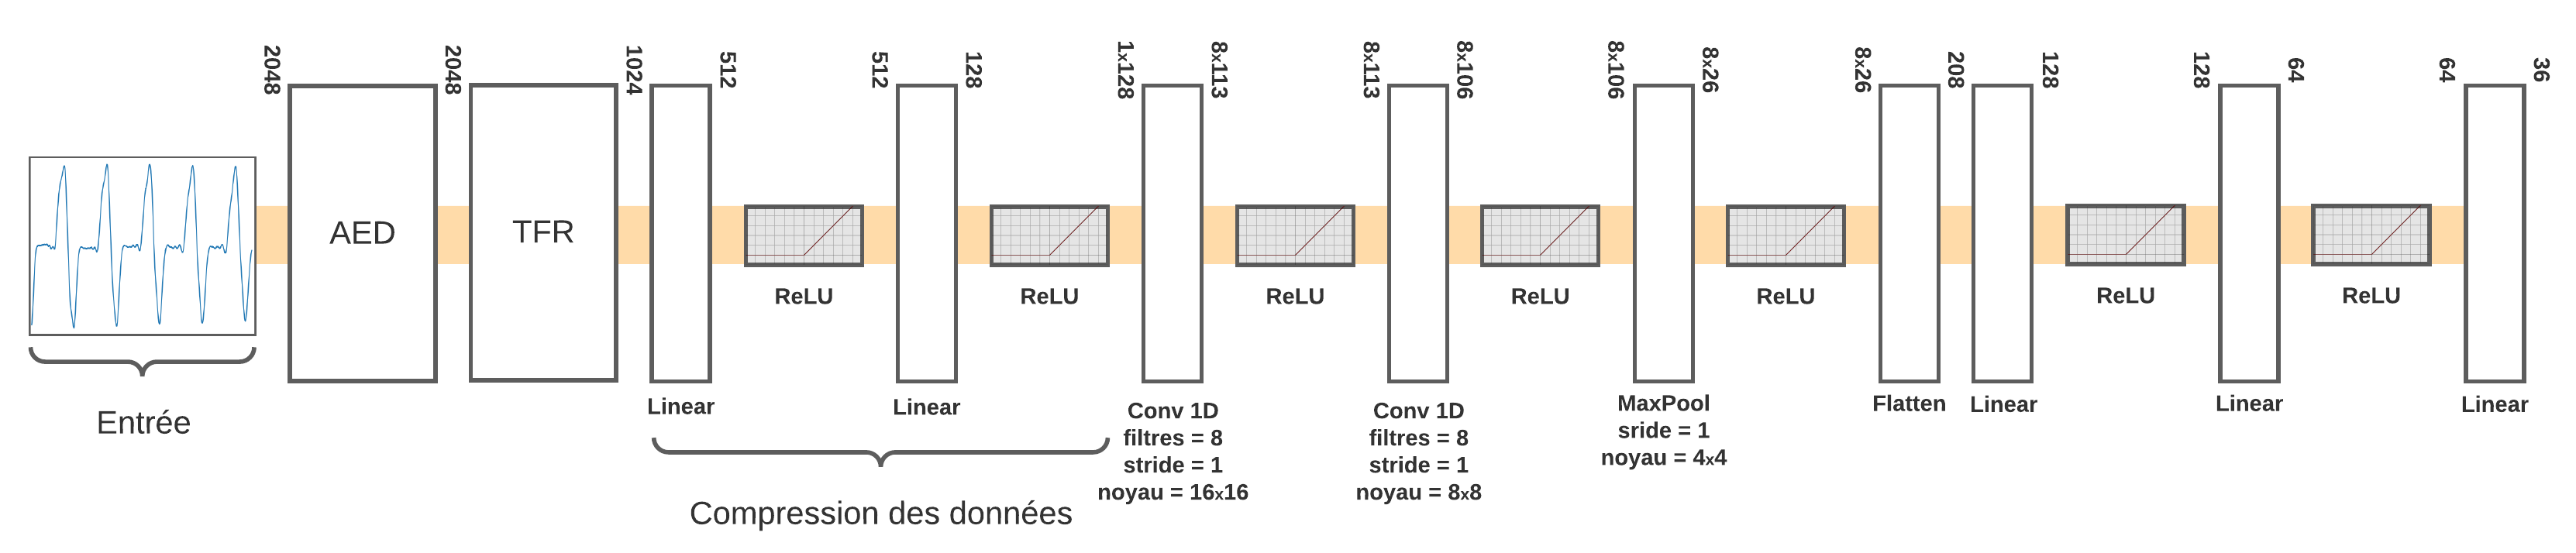
\includegraphics[width=1\linewidth]{cnn_fft}
	\caption[Architecture RNC avec TFR]{Architecture RNC avec TFR. Source : Réalisé par \textsc{Küenzi} Jean-Daniel}
	\label{fig:cnn_fft}
\end{figure}

\subsection{Matrice de confusion sur l'ensemble de validation}
\label{subsec:6.2.2}

La matrice de confusion suivante a été réalisée avec le modèle utilisant une fenêtre de 2048 échantillons.

\begin{figure}[H]
	\centering
	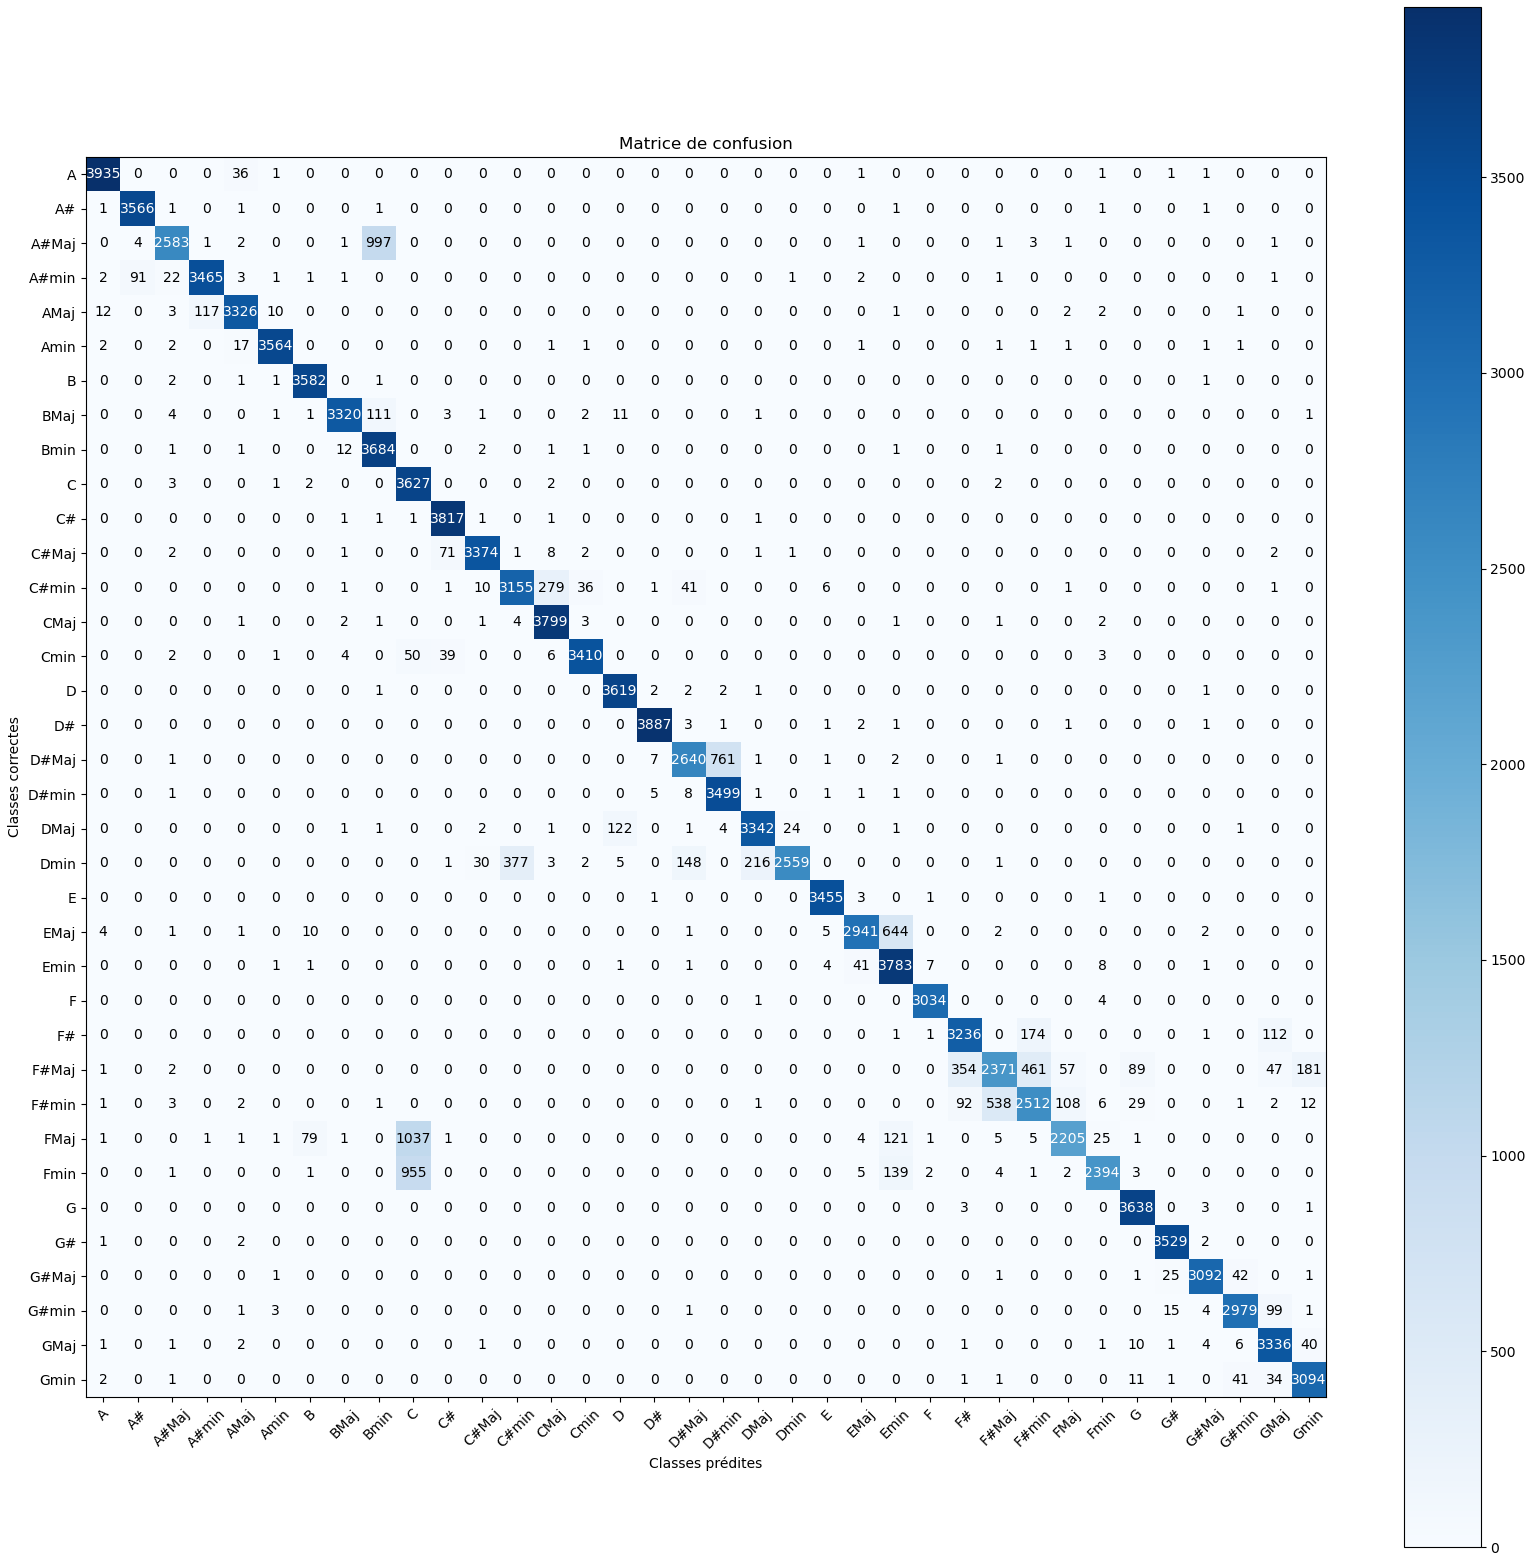
\includegraphics[width=1\linewidth]{cm_cnn_fft}
	\caption[Matrice de confusion pour l'architecture RNC avec TFR]{Matrice de confusion pour l'architecture RNC avec TFR. Source : Réalisé par \textsc{Küenzi} Jean-Daniel}
	\label{fig:cm_cnn_fft}
\end{figure}

Pour la matrice de confusion de l'architecture \gls{rnc}, on peut tout d'abord constater le même problème que celui décrit dans la \autoref{subsec:6.1.2}. Mais en plus de cela, on remarque que le modèle s'est plus trompé sur les différentes notes et accords. Notamment Dmin dont il a prédit certains exemples comme étant C\sh Maj. On peut donc observer la structure des deux accords pour essayer de comprendre ce qui s'est passé.

\begin{table}[H]
	\centering{
		\begin{tabular}{|l|c|c|}
			\hline
			& \textbf{C\sh Maj} & \textbf{Dmin} \\
			\hline
			Fondamentale & C\sh & D \\
			\hline
			Tierce & F & F \\
			\hline
			Quinte juste & G\sh & A \\
			\hline 
		\end{tabular}
		\caption[Comparaison de l'accord C\sh Maj et Dmin]{Comparaison de l'accord C\sh Maj et Dmin. Source : Réalisé par \textsc{Küenzi} Jean-Daniel}
		\label{tab:almost_same_chord}
	}
\end{table}

Dans mon ensemble de données, il se trouve que C\sh Maj et Dmin sont dans la même octave, on peut donc en déduire qu'ils partagent la même tierce, à savoir F mais aussi que la fondamentale et la quinte de l'accord Dmin sont $1/2$ ton plus élevé que celle de l'accord C\sh Maj. On peut dès lors représenter ces notes par leurs valeurs de fréquences (en Hertz) plutôt que leurs noms afin d'observer les écarts entre les fréquences de ces deux accords.

\begin{table}[H]
	\centering{
		\begin{tabular}{|l|c|c|c|}
			\hline
			& \textbf{C\sh Maj} & \textbf{Dmin} & \textbf{Écart en [Hz]} \\
			\hline
			Fondamentale [Hz] & 138.59 & 146.83 & 8.24 \\
			\hline
			Tierce [Hz] & 349.23 & 349.23 & 0.00 \\
			\hline
			Quinte juste [Hz] & 207.65 & 220 & 12.35 \\
			\hline 
		\end{tabular}
		\caption[Comparaison de l'accord C\sh Maj et Dmin sous forme de fréquences]{Comparaison de l'accord C\sh Maj et Dmin sous forme de fréquences. Source : Réalisé par \textsc{Küenzi} Jean-Daniel. A partir de \textit{Wikipedia}, ref. URL11}
		\label{tab:almost_same_chord_hz}
	}
\end{table}

Finalement cette erreur n'est pas si grave et plutôt intéressante, car on voit bien que les deux accords sont relativement proches et que peu de Hertz suffisent à les différencier. On comprend donc bien qu'avec une fenêtre de 2048 échantillons, soit une résolution fréquentielle de \textasciitilde$21.53$[Hz], nous ne sommes pas du tout précis lorsque nous effectuons la \gls{tfr} et que dans ce cas, le modèle a de la peine à bien différencier les deux accords à cause de leurs proximités. Vous pouvez retrouver en annexe (voir \autoref{app:5}) la comparaison du spectre de Fourier entre C\sh Maj et Dmin.

\subsection{Entrainements pour différentes tailles de fenêtres}

\begin{table}[H]
	\centering{
		\begin{tabular}{c l c c}
			\hline
			\multicolumn{4}{c}{\textbf{RNC avec \gls{tfr}}} \\
			\multicolumn{4}{c}{epochs = 50, $\eta$ = 0.005, nombre d'entrainements = 10} \\
			\hline
			\textbf{Nombre d'échantillons} & \textbf{Données} & \textbf{Précision moyenne \%} & \textbf{Ecart type \%} \\
			\hline
			\multirow{2}{*}{1024} & Entrainement & 99.00 & 0.35 \\
			& Validation & 86.08 & 0.78 \\
			\hline
			\multirow{2}{*}{2048} & Entrainement & 99.81 & 0.01 \\
			& Validation & 93.37 & 0.42 \\
			\hline
			\multirow{2}{*}{3072} & Entrainement & 99.82 & 0.06 \\
			& Validation & 94.30 & 0.39 \\
			\hline
			\multirow{2}{*}{4096} & Entrainement & 99.91 & 0.02 \\
			& Validation & 93.51 & 0.13 \\
			\hline
		\end{tabular}
		\caption[Entrainement de l'architecture RNC avec TFR]{Entrainement de l'architecture RNC avec TFR. Source : Réalisé par \textsc{Küenzi} Jean-Daniel}
		\label{tab:rnc_with_tfr}
	}
\end{table}

En observant ces résultats, on constate tout d'abord que l'architecture \gls{rnc} avec \gls{tfr} est légèrement moins précise que l'architecture \gls{pmc} avec \gls{tfr}. On remarque aussi qu'une fenêtre de 2048 échantillons n'est pas suffisante, l'architecture \gls{rnc} a plutôt besoin d'une fenêtre de 3072 pour atteindre sa précision maximale. Même si les résultats sont légèrement moins bons que l'architecture \gls{pmc} avec \gls{tfr}, ils restent néanmoins plutôt corrects et intéressants. Donc 3072 échantillons semblent une bonne de taille fenêtre pour avoir une bonne précision, nous avons une résolution fréquentielle de \textasciitilde$14.35$[Hz] et une résolution temporelle de \textasciitilde$0.069$[s]. Toutefois, sa résolution temporelle est un peu élevée et la latence visuelle se fait un peu ressentir lors de l'utilisation en temps réel. Généralement, en dessous de \textasciitilde0.025[s] l'œil ne perçoit pas la latence. Il vaut mieux donc utiliser une fenêtre de 2048 échantillons même si nous perdons un peu en précision afin de ne pas gêner l'utilisation en temps réel.

\begin{table}[H]
	\centering{
		\begin{tabular}{c l c c}
			\hline
			\multicolumn{4}{c}{\textbf{RNC sans \gls{tfr}}} \\
			\multicolumn{4}{c}{epochs = 50, $\eta$ = 0.005, nombre d'entrainements = 10} \\
			\hline
			\textbf{Nombre d'échantillons} & \textbf{Données} & \textbf{Précision moyenne \%} & \textbf{Ecart type \%} \\
			\hline
			\multirow{2}{*}{1024} & Entrainement & 99.49 & 0.18 \\
			& Validation & 90.28 & 0.41 \\
			\hline
			\multirow{2}{*}{2048} & Entrainement & 99.84 & 0.04 \\
			& Validation & 91.51 & 0.42 \\
			\hline
			\multirow{2}{*}{3072} & Entrainement & 99.89 & 0.05 \\
			& Validation & 90.78 & 0.30 \\
			\hline
			\multirow{2}{*}{4096} & Entrainement & 99.85 & 0.06 \\
			& Validation & 89.54 & 0.58 \\
			\hline
		\end{tabular}
		\caption[Entrainement de l'architecture RNC sans TFR]{Entrainement de l'architecture RNC sans TFR. Source : Réalisé par \textsc{Küenzi} Jean-Daniel}
		\label{tab:rnc_without_tfr}
	}
\end{table}

En observant ces résultats, on constate tout d'abord que l'architecture \gls{rnc} sans \gls{tfr} est moins précise que l'architecture \gls{pmc} sans \gls{tfr}. On constate également que la fenêtre avec 2048 échantillons est celle qui a donné les meilleurs résultats. Finalement on peut observer qu'à partir de la fenêtre avec 2048 échantillons, l'augmentation du nombre d'échantillons fait chuter la précision du modèle. Cela est surement dû aux mêmes raisons que pour l'architecture \gls{pmc} sans \gls{tfr}.

Finalement, l'architecture convolutive est celle qui a donné les moins bons résultats, c'est pourquoi je ne l'ai pas retenue comme ma solution finale. Toutefois, ses résultats restent corrects et encourageants, cette architecture n'est donc pas à négliger.